\chapter{Evaluación}

En este capítulo se analizará el escenario implementado con los distintos dispositivos explicados a lo largo de la documentación. El objetivo es ver si con una Raspberry Pi se puede realizar este escenario o a mayor escala.

Por recordar, los elementos utilizados son los siguientes:

\begin{itemize}
    \item Portátil Asus ROG GL752VW con un i7-6700HQ y 24GB de memoria RAM
    \item Raspberry Pi modelo 3B con 1GB de RAM
    \item 2 Microcontroladores ESP32
\end{itemize}

En la implementación, en la sección sobre el fichero de ejecución de múltiples nodos, este es ejecutado en el portátil mencionado para las diferentes pruebas. 

En este caso se va a realizar otro archivo diferente, que agrupe los nodos de \textit{Controlador}, \textit{Base de Datos} y los contenedores que actúan como agentes de microROS para recopilar y publicar la información en el dominio utilizado.

El objetivo es ver el consumo de memoria por parte de los procesos anteriores ejecutados en la Raspberry Pi.

Para ver si se producen cambios en la memoria si hay más o menos nodos en la red, estos serán ejecutados en el portátil mencionado.

\section{Escenario 1}

Se va a ejecutar un único fichero, el nodo Controlador en la Raspberry Pi, para ello se verá la memoria antes y después de la ejecución. El comando a utilizar va a ser \textit{free -h} que nos devuelve el uso de esta dividida en las diferentes cabeceras.

\begin{center}
    \centering
    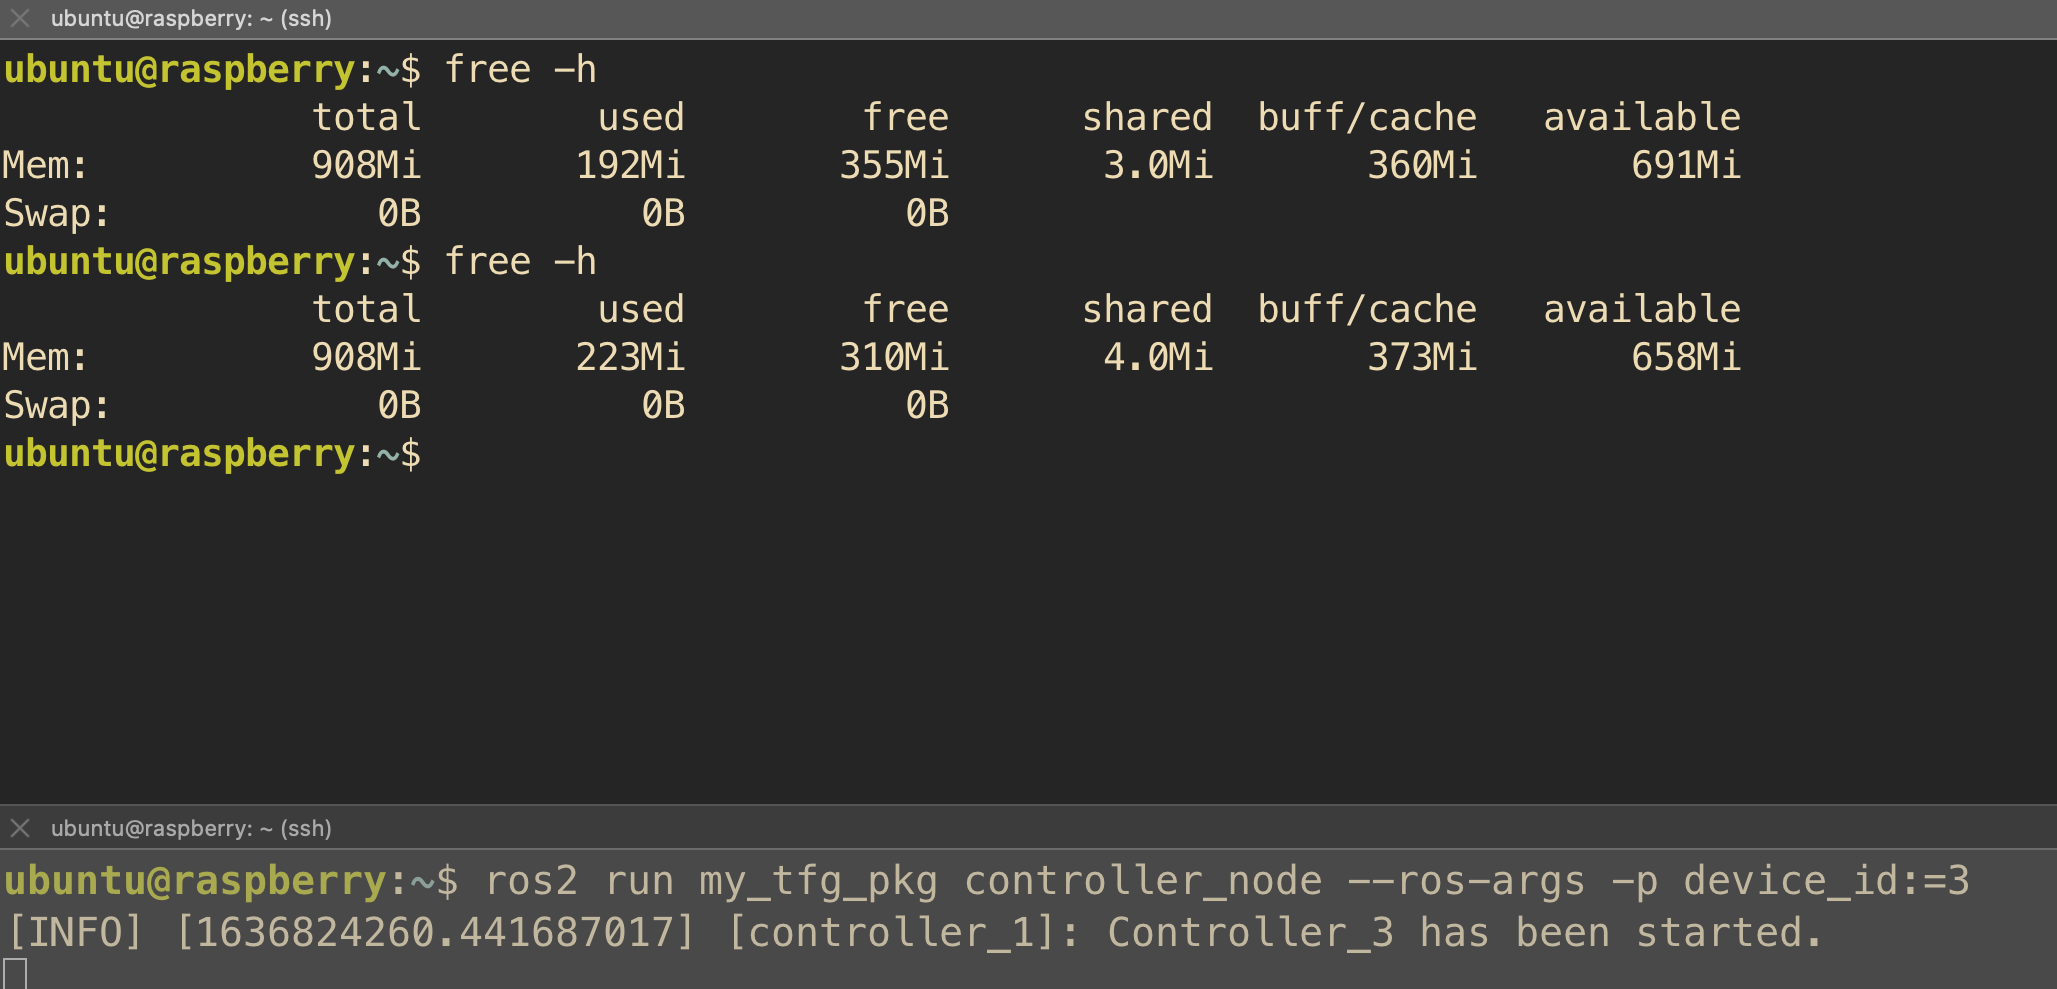
\includegraphics[width=\textwidth]{img/09-Escenario1.png}
    \captionof{figure}{Escenario 1}
    \label{fig:escenario-1}
\end{center}

En la figura \ref{fig:escenario-1} se puede observar dos ejecuciónes para medir la memoria en la parte superior, una ejecutada antes y otra después de la llamada al nodo controlador. Por tanto el consumo de memoria producido en este caso es de 41MB. 

Tras la ejecución de este escenario unas 5 veces, el consumo de memoria se ha mantenido igual, variando 1MB en algunos casos, pudiendo ser debido a otro proceso del sistema.

\section{Escenario 2}

En este caso se han lanzado diferentes nodos en la Raspberry Pi, el Controlador y el gestor de la base de datos. Al igual que en el caso anterior, se va a medir la memoria con \textit{free -h} en el mismo formato:

\newpage

\begin{center}
    \centering
    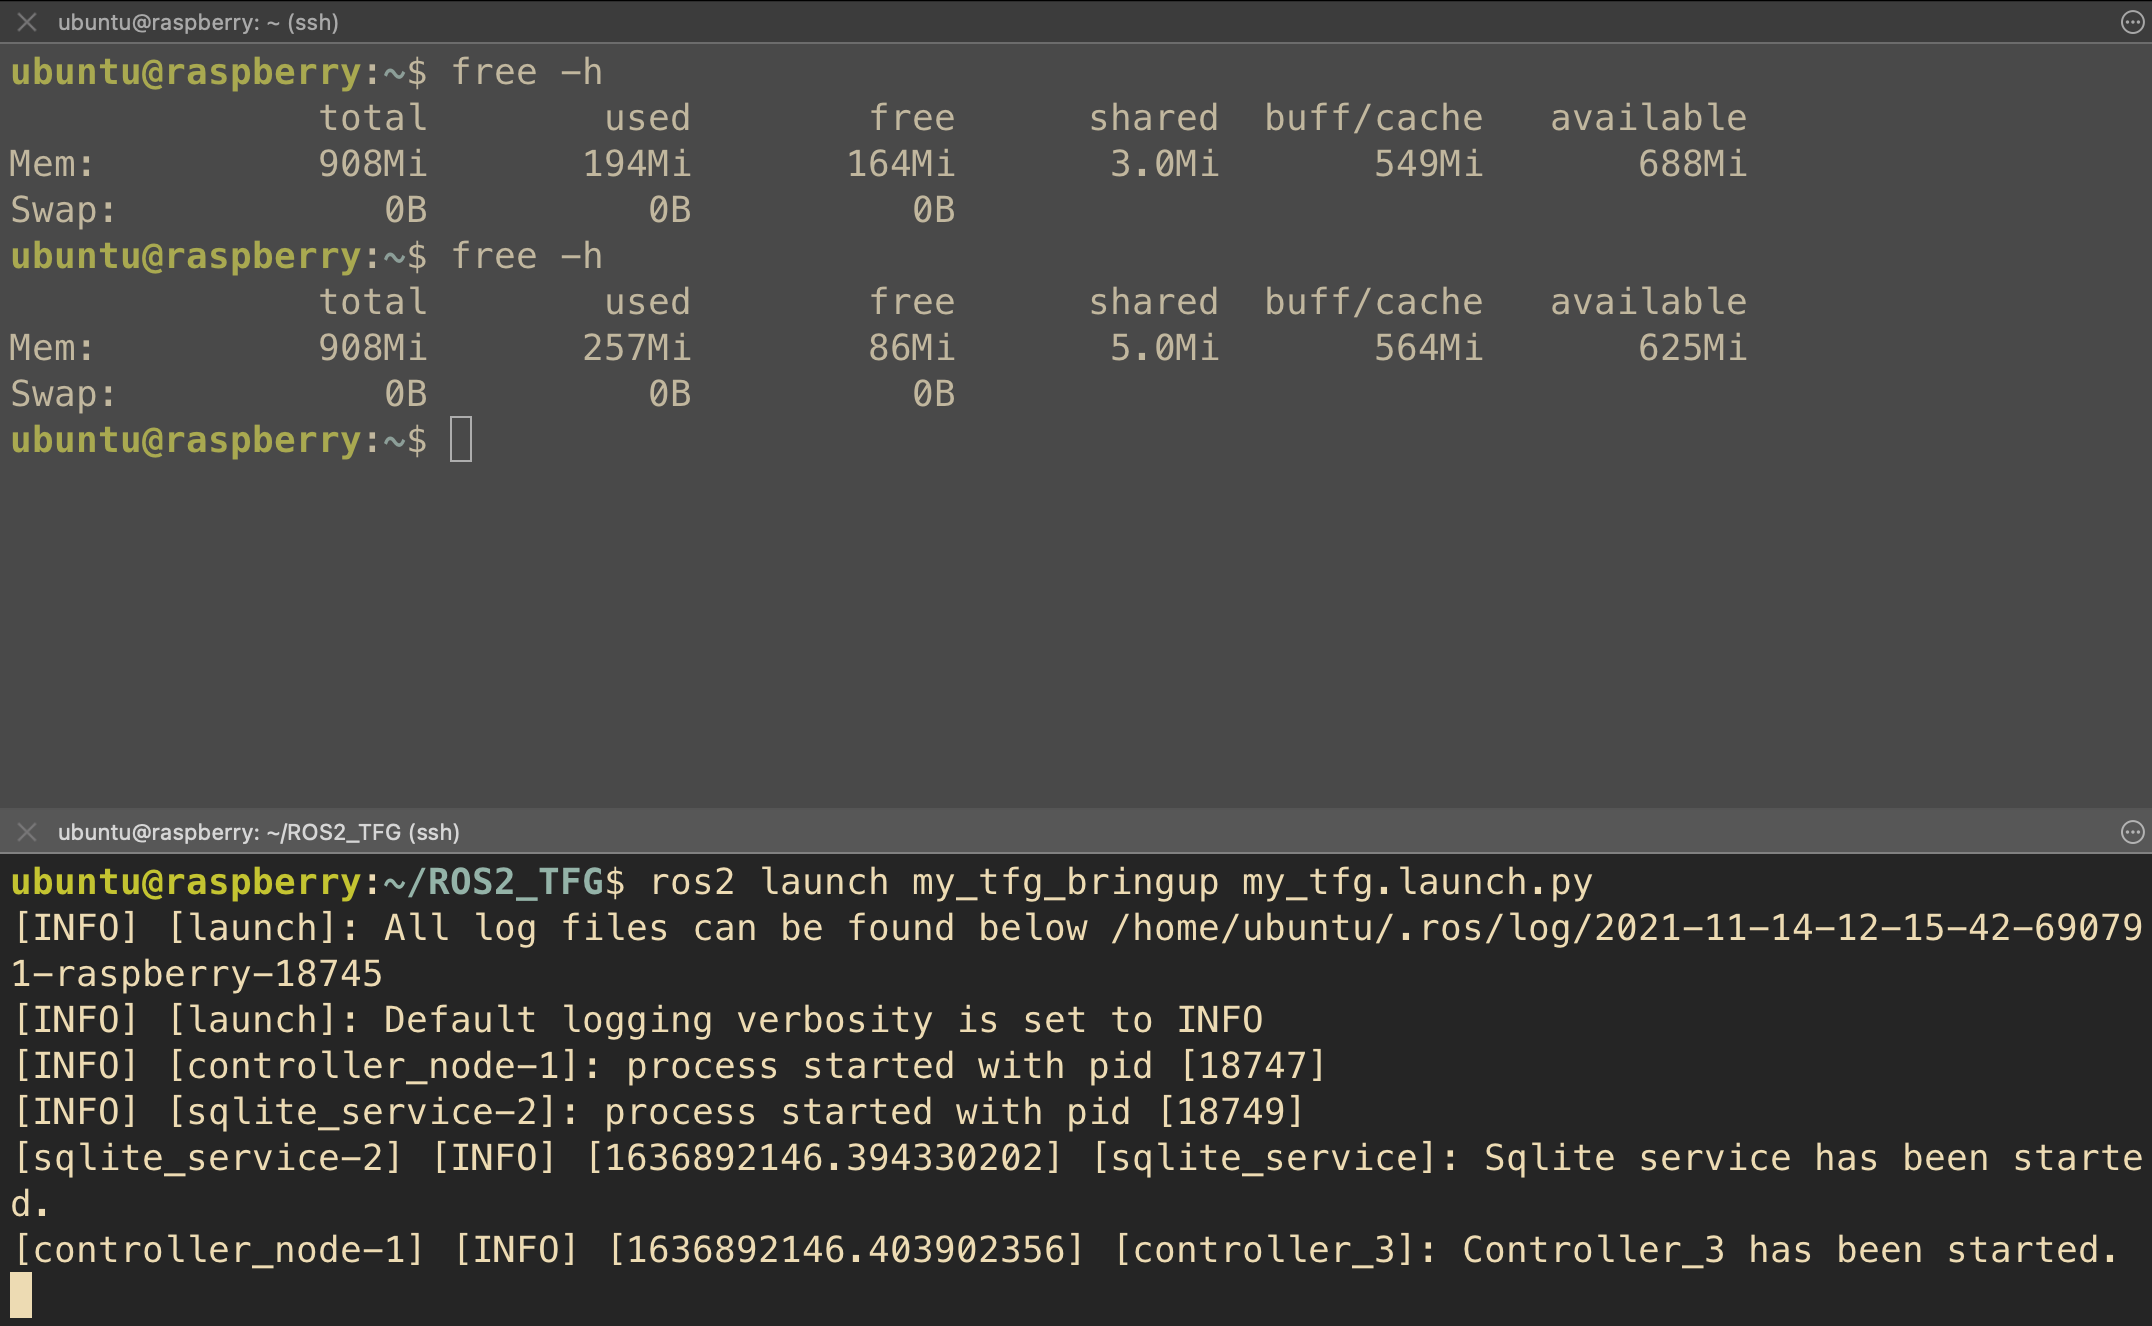
\includegraphics[width=\textwidth]{img/09-Escenario2.png}
    \captionof{figure}{Escenario 2}
    \label{fig:escenario-2}
\end{center}

Como se puede observar, el consumo de la memoria ha aumentado respecto al anterior ya que se están ejecutando actualmente dos nodos, siendo este de 63MB al ser ejecutado.

\section{Escenario 3}

Por último, se van a lanzar todos los nodos mostrados en la figura \ref{fig:rqt-graphs} en el capítulo de implementación. Además de esos, estará la Raspberry Pi 3B con los nodos en ejecución, para ver si se refleja toda la comunicación en la memoria. Esta parte será la mostrada en la terminal, ya que es la memoria que se está analizando.

\newpage

\begin{center}
    \centering
    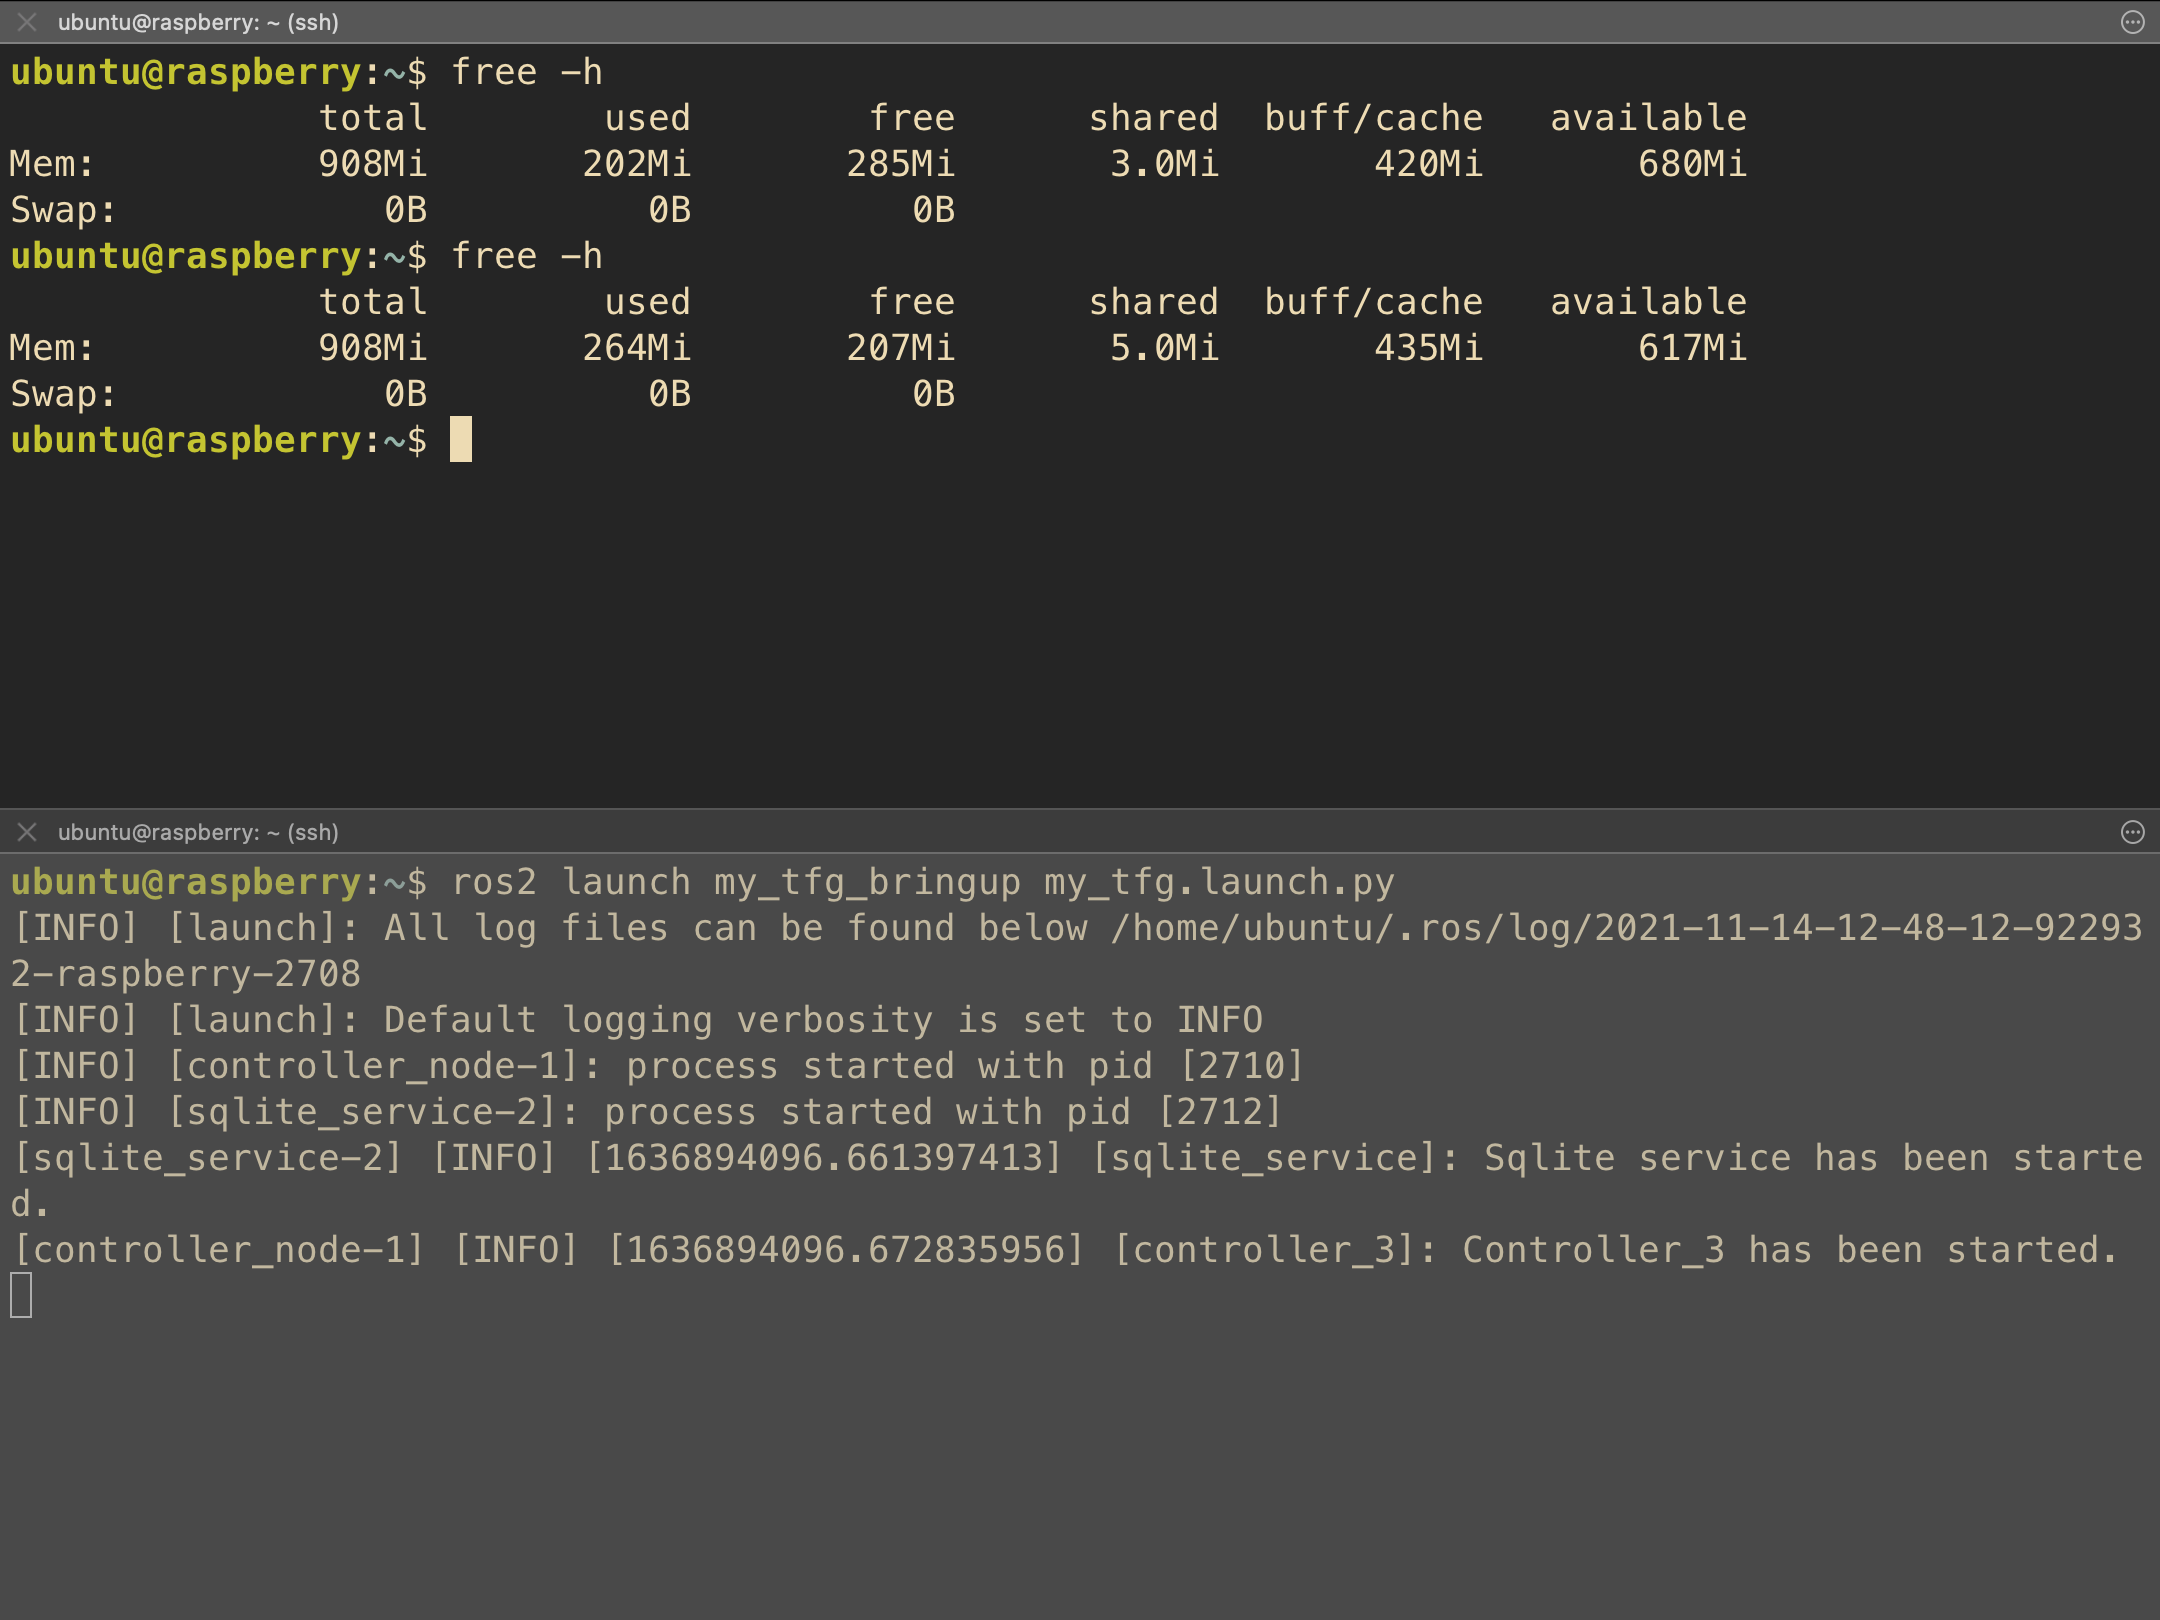
\includegraphics[width=\textwidth]{img/09-Escenario3.png}
    \captionof{figure}{Escenario 3}
    \label{fig:escenario-3}
\end{center}

Al igual que en el escenario 2, el consumo de memoria mostrado en la figura \ref{fig:escenario-3} es de 63MB.

Por comprobar esta variación, se ha ejecutado este escenario 5 veces, obteniendo los casi mismos resultados en las diferentes ocasiones, mostrado en la siguiente tabla:


\begin{center}
\begin{tabular}{||c c c c||} 
 \hline
  & Memoria Inicial & Memoria en ejecución & Memoria consumida \\ [0.5ex] 
 \hline\hline
 1 & 680 & 617 & 63 \\ 
 \hline
 2 & 685 & 623 & 62 \\
 \hline
 3 & 686 & 623 & 63 \\
 \hline
 4 & 685 & 623 & 62 \\ 
 \hline
 5 & 685 & 623 & 62 \\


 \hline
\end{tabular}
\captionof{figure}{Tabla de Temperatura}
\end{center}

Para poder analizar el estado de la red de los diferentes nodos, se va a mostrar un gráfico utilizando el programa rqt\_graph.

\begin{center}
    \centering
    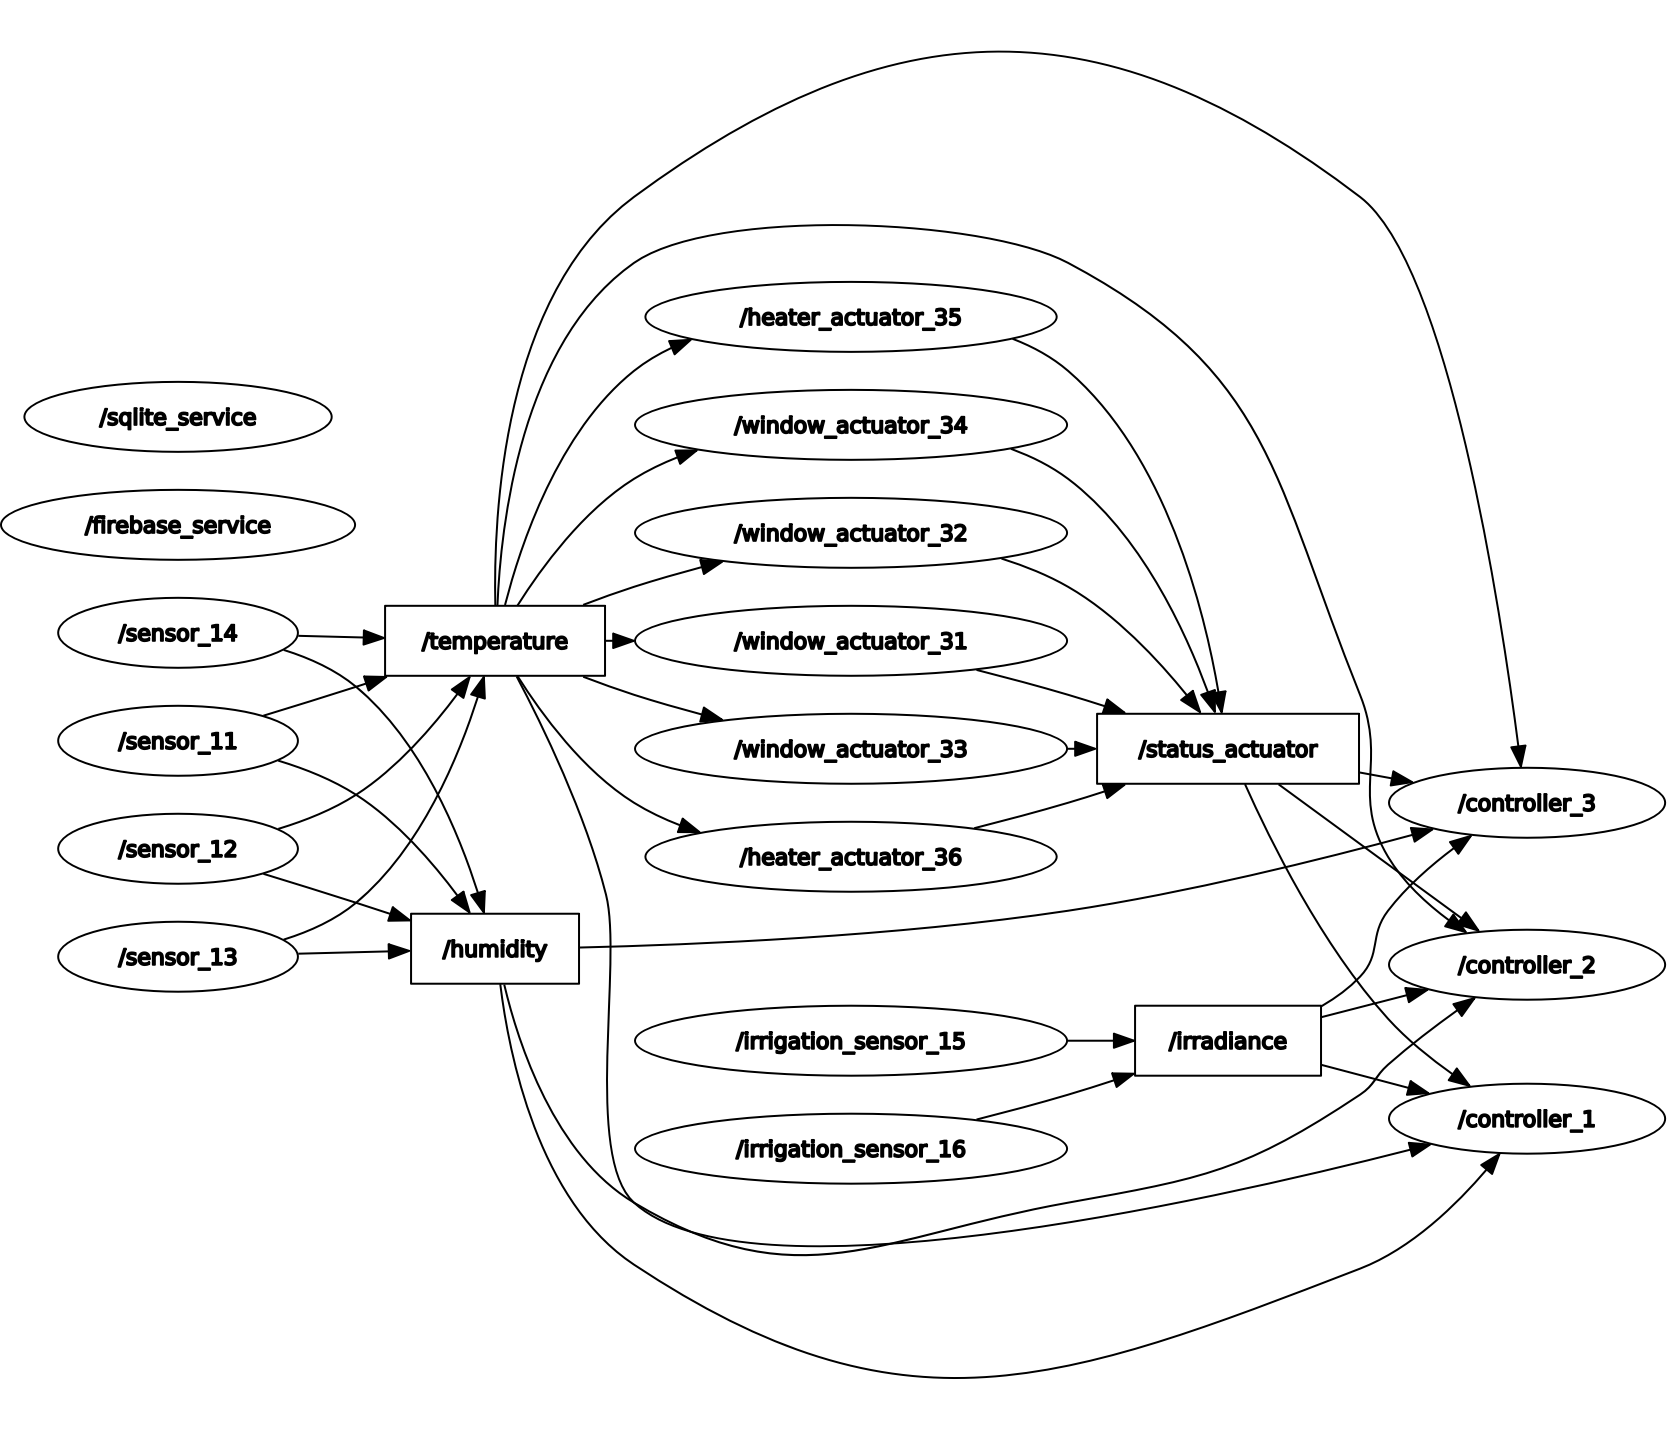
\includegraphics[width=\textwidth]{img/09-Escenario-3-rosgraph.png}
    \captionof{figure}{Red en el Escenario 3}
    \label{fig:rqt-escenario-3}
\end{center}

Por aclarar este escenario, al igual que se ha explicado en el diagrama del análisis \ref{fig:diagrama-comunicacion-nodos} y en la implementación \ref{fig:rqt-graphs}, los rectángulos representan los tópicos y los óvalos representan los diferentes nodos.

Para especificar donde se estaba ejecutando cada nodo, se va a listar a continuación:

\begin{itemize}
    \item Las placas ESP32 están representadas con \textbf{sensor\_11} y \textbf{sensor\_12}
    \item La Raspberry Pi 3B utilizada durante todo el escenario está ejecutando los nodos \textbf{controller\_3} y \textbf{sqlite\_service}
    \item El portátil Asus esta ejecutando los demás dispositivos de manera virtual.
\end{itemize}

Finalizando esta sección, se ha utilizado Wireshark \cite{wireshark} para capturar el tráfico generado en la red. 

Tras dejar el sistema durante 30 minutos en ejecución, se ha aplicado como filtro que el protocolo utilizado sea RTPS, ya que es utilizado en la comunicación entre los diferentes nodos.

Con la funcionalidad de Stadistics ofrecida por Wireshark, se ha obtenido una gráfica mostrando la cantidad de paquetes cada 10 segundos, representado en la siguiente imagen:

\begin{center}
    \centering
    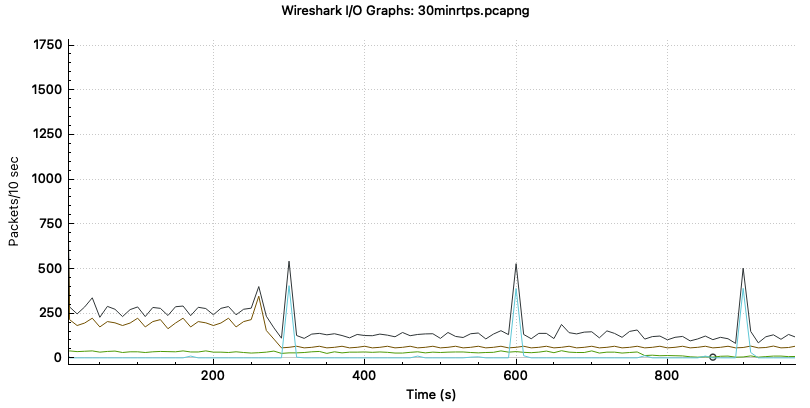
\includegraphics[width=\textwidth]{img/09-30minrtps.png}
    \captionof{figure}{Gráfica generada por Wireshark}
    \label{fig:wireshark-30min}
\end{center}

Como se puede observar, hay varias líneas mostradas en el gráfico:

\begin{itemize}
    \item La marrón es el protocolo RTPS
    \item La verde es el protocolo ARP
    \item La azul es el protocolo TCP
    \item La negra es el número de paquetes total
\end{itemize}

Cada cierto tiempo, se produce un pico de paquetes en la red se vuelve a estabilidad. Esto es debido al almacenamiento de los datos en la plataforma de Firebase, que se ejecuta cada ese periodo, establecido con un temporizador.

Por lo tanto se podría concluir que la cantidad de paquetes es estable respecto a RTPS una vez pasado un tiempo desde que comienza la red, y la comunicación con la base de datos cada este periodo produce esos picos.